\documentclass[12pt,a4paper,titlepage,openany,twoside]{report}
\usepackage{magistrska_FAMNIT_2_stopnja_MA_MEF_2021}
\usepackage{import}
\usepackage{listings}
\usepackage{comment}
\usepackage{csquotes}
\usepackage{xcolor} 
\usepackage{transparent}
\definecolor{mred}{RGB}{255,100,103}
\definecolor{mblue}{RGB}{81,162,255}
\definecolor{mgreen}{RGB}{5,233,114}
\definecolor{mgrey}{RGB}{150,150,150}
\usepackage[inkscapelatex]{svg}
%%%%%%%%%%%%%%%%%%%%%    BP  %%%%%%%%%%%%%%%%%%%%

\newcommand{\Rang}[3]{%
  \ensuremath{ \mathop{rang}_{#1}(#2,#3) }% rang
}

\newcommand{\Izbira}[3]{%
  \ensuremath{ \mathop{Izbira}_{#1}(#2,#3)} % izbira
}

\newcommand{\Popcount}[1]{%
  \ensuremath{ \mathop{\texttt{popcount}}\left(#1\right) }% pop count
}

\newcommand{\Predhodnik}[3]{%
  \ensuremath{ \mathop{predhodnik}_{#1}(#2,#3) }% Predhodnik
}

\newcommand{\Naslednik}[3]{%
  \ensuremath{ \mathop{naslednik}_{#1}(#2,#3) }% Naslednik
}

\newcommand{\Visek}[2]{%
  \ensuremath{ \mathop{\textit{višek}}(#1,#2) }% Višek
}
\newcommand{\visek}[3]{%
  \ensuremath{ \mathop{\textit{višek}}(#1,#2,#3) }% Relativni višek intervala
}
\newcommand{\rmq}[3]{%
  \ensuremath{ \mathop{rmq}(#1,#2,#3) }% rmq
}
\newcommand{\rMq}[3]{%
  \ensuremath{ \mathop{rMq}(#1,#2,#3) }% rMq
}

\newcommand{\MinStetje}[3]{%
  \ensuremath{ \mathop{\textit{inŠtetje}}(#1,#2,#3) }% Min štetje
}

\newcommand{\MinIzbira}[4]{%
  \ensuremath{ \mathop{\textit{minIzbira}}(#1,#2,#3,#4) }% Min izbira
}

%%%%%%%%%%%%%%%%%%%%%    KOmpaktna drevesa  %%%%%%%%%%%%%%%%%%%%

\newcommand{\Zapri}[2]{%
  \ensuremath{ \mathop{zapri}(#1,#2) }% Zapri ukleaj
}

\newcommand{\Odpri}[2]{%
  \ensuremath{ \mathop{odpri}(#1,#2) }% Odpri zaklepaj
}
\newcommand{\IskanjeNAprej}[3]{%
  \ensuremath{ \mathop{iskanjeNapre}(#1,#2,#3) }% Iskanje naprej
}

\newcommand{\Oklepa}[2]{%
  \ensuremath{ \mathop{oklepa}(#1,#2) }% Oklepaja ki oklepata
}

%%%%%%%%%%%%%%%%%%%%%    DREVESA  %%%%%%%%%%%%%%%%%%%%

\newcommand{\Globina}[1]{%
  \ensuremath{ \mathop{globina}(#1) }% globina vozlišča v
} 

%%%%%%%%%%%%%%%%%%%%%    ST   %%%%%%%%%%%%%%%%%%%%

\newcommand{\Koren}{%
  \ensuremath{ \mathop{koren}() }% koren drevesa
}   

\newcommand{\List}[1]{%
  \ensuremath{\mathop{jeList}(#1) }% vrne, ali je v list
} 

\newcommand{\Otrok}[2]{%
  \ensuremath{\mathop{otrok}(#1,#2) }% vrne, i-tega otroka od v 
} 

\newcommand{\PrviOtrok}[1]{%
  \ensuremath{\mathop{prviOtrok}(#1) }% vrne, prvega otroka od v
} 

\newcommand{\PBrat}[1]{%
  \ensuremath{\mathop{pBrat}(#1) }% vrne, vrne predhonjega brata od v
} 

\newcommand{\NBrat}[1]{%
  \ensuremath{\mathop{nBrat}(#1) }% vrne, vrne naslednjega brata od v
} 

\newcommand{\Stars}[1]{%
  \ensuremath{\mathop{\textit{starš}}(#1) }% vrne, vrne naslednjega brata od v
} 

\newcommand{\Povezava}[2]{%
  \ensuremath{\mathop{povezava}(#1,#2) }% vrne, vrne naslednjega brata od v
} 

\newcommand{\Sd}[1]{%
  \ensuremath{ \mathop{sd}(#1) }% črkovna globina vozlišča v
}  


\newcommand{\Lca}[2]{%
  \ensuremath{ \mathop{lca}(#1,#2) } % najnglobji skupni predhodnik
}  

\newcommand{\Sl}[1]{%
  \ensuremath{ \mathop{sl}(#1) }% priponska povezava od v
} 


%%%%%%%%%%%%%%%%%%%%%    Poizvedbe  %%%%%%%%%%%%%%%%%%%%

\newcommand{\Prisotnost}[2]{%
  \ensuremath{ \mathop{prisotnost}(#1,#2) }% prisotnost vzorca P v besedilu T
} 

\newcommand{\SteviloPonovitev}[2]{%
  \ensuremath{ \mathop{\textit{številoPonovitev}}(#1,#2) }% število ponovitev vzorca P v besedilu T
} 

\newcommand{\SeznamPojavov}[2]{%
  \ensuremath{ \mathop{\textit{seznamPojavov}}(#1,#2) }% število ponovitev vzorca P v besedilu T
} 

%%%%%%%%%%%%%%%%%%%%%   SA  %%%%%%%%%%%%%%%%%%%%

\newcommand{\lcp}[2]{%
  \ensuremath{ \mathop{lcp}(#1,#2) }% LCP med dvemi besedami
} 

\newcommand{\lInterval}[3]{%
  \ensuremath{ [#1,#2] #3-interval }% l interval
}

%%%%%%%%%%%%%%%%%%%%%   CSA  %%%%%%%%%%%%%%%%%%%%

\newcommand{\Pripona}[1]{%
  \ensuremath{ \mathop{pripona}(#1) }% pripona na item mestu 
} 

\newcommand{\Inverz}[1]{%
  \ensuremath{ \mathop{inverz}(#1) }% pozicija pripone , ki se začne z i-tim znakom
} 

\newcommand{\PsiFunkcija}[1]{%
  \ensuremath{ \mathop{\Psi}(#1) }% psi funkcija od i
} 

\newcommand{\Beseda}[2]{%
  \ensuremath{ \mathop{beseda}(#1,#2) }% izpis prvih d znakov pripone na i-tem mestu
} 


%%%%%%%%%%%%%% prazne vrstice %%%%%%%%%%%%%%%%%%%%%%%%%


\graphicspath{./Slike/}

% Glava dokumenta:

\fancyhf{}
\lhead[{\fontsize{9.3}{12}\selectfont
Suban J. Kompaktna priponska drevesa.\\ %Spremeni naslov dela
\noindent Univerza na Primorskem, Fakulteta za matematiko, naravoslovje in informacijske tehnologije, 2025}]{{\fontsize{9.3}{12}\selectfont
Suban J. Kompaktna priponska drevesa.\\ %Spremeni naslov dela
\noindent Univerza na Primorskem, Fakulteta za matematiko, naravoslovje in informacijske tehnologije, 2025}}
\chead[]{\fancyplain{}{}}
\rhead[\fancyplain{\thepage}{\thepage}]{\fancyplain{\thepage}{\thepage}}
\cfoot[]{\fancyplain{}{}}
\lfoot[]{\fancyplain{}{}}
\rfoot[]{\fancyplain{}{}}
\normalsize

%%%%%%%%%%%%%%%%%%%%%%%%% ZAČETEK DOKUMENTA %%%%%%%%%%%%%%%%%%%%%%%%%%%%%%%%%%%%%%%%%%5

%%%%%%%%%%%%%%%%%%%%%%%%% Naslovna stran %%%%%%%%%%%%%%%%%%%%%%%%%


\begin{document}
\pagenumbering{Roman}
\pagestyle{empty}
\begin{center}
\noindent \large UNIVERZA NA PRIMORSKEM\\
\large FAKULTETA ZA MATEMATIKO, NARAVOSLOVJE IN\\
INFORMACIJSKE TEHNOLOGIJE


\normalsize
\vspace{6cm}
Magistrsko delo\\
\textbf{\large Kompaktna priponska drevesa}\\ %Spremeni naslov dela
\normalsize
(Compact Suffix Tree)\\ %Spremeni naslov dela v angleščini
\end{center}

\begin{flushleft}
\vspace{5cm}
\noindent Ime in priimek: \textit{Jani Suban}
% v zgornjo vrstico dopišite ime in priimek študenta
\\
\noindent Študijski program: \textit{Računalništvo in informatika, 2. stopnja}
% v zgornjo vrstico dopišite ime študijskega programa
\\
\noindent Mentor: \textit{prof. dr. Andrej Brodnik}
% v zgornjo vrstico dopišite akademski naziv, ime in priimek mentorja
\\
\noindent Somentor: \textit{izr. prof. dr. Rok Požar}
% če imate somentorja, v zgornjo vrstico dopišite akademski naziv, ime in priimek somentorja
% če somentorja nimate, zbrišite zgornjo in spodnjo vrstico
\\

\end{flushleft}

\vspace{4cm}
\begin{center}
\large {Koper, april 2025} %spremeni mesec oddaje
% dopišite mesec in leto oddaje zaključne naloge
\end{center}
\newpage

\pagestyle{fancy}
%%%%%%%%%%%%%%%%%%%%%%%%%%%%%%% Ključna dokumentacijska informacija (slo in ang) %%%%%%%%%%%

\subsubsection*{\textbf{Ključna dokumentacijska informacija}}
\vspace{-0.7cm}
%\medskip
\begin{center}
\fbox{\parbox{\linewidth}{
%\vspace{0.2cm}
\noindent
Ime in PRIIMEK: Jani SUBAN  \\%\vspace{0.5cm}\\
Naslov magistrskega dela: Kompaktna priponska drevesa\vspace{0.5cm}\\ %Dodaj naslov dela
Kraj: Koper \\%\vspace{0.5cm}\\
Leto: 2025\vspace{0.5cm}\\
Število listov: 73 \hspace{2cm} Število slik: 17 \hspace{2.6cm} Število tabel: 6\hspace{2cm} \\ %\vspace{0.5cm}\\
%Število prilog: \hspace{1.9cm} Število strani prilog: \hspace{1cm} \\
Število referenc: 21\\ %\vspace{0.5cm}\\
Mentor: prof. dr. Andrej Brodnik \\
Somentor: izr. prof. dr. Rok Požar\vspace{0.5cm}\\
UDK: \\
Ključne besede:\\ %\vspace{0.5cm}\\
POPRAVI: Math.~Subj.~Class.~(2010):\\ %\vspace{0.5cm}\\ %Spremeni ključne besede
Izvleček:\\
POPRAVI:: Izvleček predstavlja kratek, a jedrnat prikaz vsebine naloge. V največ 250 besedah nakažemo problem, metode, rezultate, ključne ugotovitve in njihov pomen.
%\vspace{0.2cm} %spremeni izvleček
}}
\end{center}

\newpage

\subsubsection*{\textbf{Key document information}}
\vspace{-0.7cm}
%\medskip

\begin{center}
\fbox{\parbox{\linewidth}{
%\vspace{0.2cm}
\noindent
Name and SURNAME: Jani SUBAN \\%\vspace{0.5cm}\\
Title of the thesis: Compressed Suffix Tree\vspace{0.5cm}\\  %Dodaj naslov dela
Place: Koper \\%\vspace{0.5cm}\\
Year: 2025\vspace{0.5cm}\\
Number of pages: 73\hspace{1.6cm} Number of figures: 17\hspace{2.2cm} Number of tables: 6\\ %\hspace{2cm}  %\vspace{0.5cm}\\
%Number of appendices: \hspace{0.6cm} Number of appendix pages: \hspace{0.8cm} \\
Number of references: 21\\ %\vspace{0.5cm}\\
Mentor: prof. dr. Andrej Brodnik\\%\vspace{0.5cm}\\
Co-Mentor: izr. prof. dr. Rok Požar\vspace{0.5cm}\\
UDC: \\
Keywords:\\ %\vspace{0.5cm}\\
Math.~Subj.~Class.~(2010):\\ %\vspace{0.5cm}\\ %spremeni ključne besede
Abstract:\\
Izvleček predstavlja kratek, a jedrnat prikaz vsebine naloge. V največ 250 besedah nakažemo problem, metode, rezultate, ključne ugotovitve in njihov pomen. %spremeni izvleček
%\vspace{0.2cm}
}}
\end{center}






%%%%%%%%%%%%%%%%%%%%%%%%%%%%% Kazala %%%%%%%%%%%%%%%%%%%%%%%%%%%%%%
\newpage

% Dodamo kazala (po potrebi):
\tableofcontents
\addtocontents{toc}{\protect\thispagestyle{fancy}}
\newpage
\listoftables
\addtocontents{lot}{\protect\thispagestyle{fancy}}
\newpage
\listoffigures
\addtocontents{lof}{\protect\thispagestyle{fancy}}
\newpage
% ker priloge niso oštevilčene, tudi pikic do številk strani (ki jih ni) ne izpišemo
%\renewcommand{\cftdot}{}
%\listofappendices
%\thispagestyle{fancy}
%\newpage

\chapter*{Seznam kratic}
\thispagestyle{fancyplain}
\import{.}{Drugo/Kratice}
\newpage

\normalsize

%%%%%%%%%%%%%%%%%%%%%%%%%%%%%%%%%% Poglavja: %%%%%%%%%%%%%%%%%%%%%%%%%%%%%%%%%%%%%

%%%%%%%%%%%%%%%%%%%%%%%%%%%%%%% Zahvala %%%%%%%%%%%%%%%%%%%%%%%%%%%%%%%%%%%%%

\newpage
\section*{\textbf{Zahvala}}


Tu se zahvalimo sodelujočim pri zaključni nalogi, osebam ali ustanovam, ki so nam pri delu pomagale ali so delo omogočile. Zahvalimo se lahko tudi mentorju in morebitnemu somentorju.


% Namig: Za večjo preglednost datoteke lahko vsebino vsakega poglavja shranite v poseben .tex dokument
% v isto mapo, kjer je shranjena osnovna .tex datoteka. Nato poglavja vstavite v dokument s klicem \include
% Primer: PrvoPoglavje.tex in DrugoPoglavje.tex vstavimo tako:
% \include{PrvoPoglavje}
% \include{DrugoPoglavje}

\chapter{UVOD}\label{sec:uvod}
\thispagestyle{fancy} % To uporabi pri vsakem \chapter, sicer ne pokaze glave dokumenta
\pagenumbering{arabic}

\import{.}{Uvod/Uvod}

\chapter{OZNAKE, DEFINICIJE IN OSNOVNE OPERACIJE}\label{sec:Notacija}
\thispagestyle{fancy} 
\import{.}{Notacija/Uvod}

\chapter{PRIPONSKA DREVESA}\label{sec:priponska_drevesa}
\thispagestyle{fancy} 
\import{.}{PriponskaDrevesa/PriponskaDrevesa}

\chapter{PRIPONSKO POLJE}\label{sec:SA}
\import{.}{PriponskoPolje/PriponskoPolje}

\chapter{KOMPAKTNA PREDSTAVITEV PRIPONSKEGA DREVESA}\label{sec:Kompaktna}
\thispagestyle{fancy} 
%\import{.}{KompaktnaPredstavitev/Uvod}

%\section{KOMPAKTNA PREDSTAVITEV DREVES}\label{sec:kompaktna_drevesa}
%\import{.}{KompaktnaPredstavitev/KompaktnaDrevesa}

%\section{KOMPAKTNA PRIPONSKA DREVESA}\label{sec:CST}
\import{.}{KompaktnaPredstavitev/KompaktnaPriponskaDrevesa}

\chapter{OPERACIJE NAD PRIPOSKIMI DREVSESI}\label{sec:OPeracije}
\thispagestyle{fancy} 
\import{.}{Operacije/Uvod}



\section{TEORETIČNA ANALIZA}\label{sec:analiza}
%\import{.}{Operacije/Analiza}
\import{.}{Operacije/AnalizaSamoTabele}


\section{OPIS METODE EMPIRIČNE PRIMERJAVE}\label{sec:opis}
\import{.}{Operacije/Opis}


\section{REZULTATI EMPIRIČNE PRIMERJAVE}\label{sec:primerjava}
\import{.}{Operacije/Evalvacija}

\chapter{ZAKLJUČEK}\label{sec:zakljucek}
\thispagestyle{fancy} 
\import{.}{Zakljucek/Zakljucek}



%\chapter{VLOŽITVE}
%\thispagestyle{fancy}
%
%Dodamo vezno besedilo.
%
%\section{ŠIROKE VLOŽITVE}\label{siroke}
%
%Dodamo vezno besedilo.
%
%\subsection{Podpoglavje poglavja Široke vložitve}
%
%Dodamo vezno besedilo.
%
%\subsubsection{Podpoglavje podpoglavja Široke vložitve}
%
%Dodamo vezno besedilo.
%
%\begin{defi}
%Graf $G$ je {\em povezan}, če za vsaki dve točki $u,v\in V(G)$ obstaja vsaj ena $u$-$v$ pot v $G$.
%\end{defi}
%
%\begin{lema}
%Lema je pomožna trditev, ki služi za dokaz glavnega izreka.
%\end{lema}
%
%\begin{proof}
%Tu napišimo dokaz leme. Dokaz naj bo čim krajši, vendar razumljiv vsem študentom. Pazite na logično strukturo dokaza: Vsi koraki naj bodo utemeljeni.
%\end{proof}
%
%\begin{izr}
%Izrek je najpomemnejša trditev v poglavju. Izrekov naj bo čim manj, preostale trditve formuliramo kot leme ali kot trditve.
%\end{izr}
%
%\begin{proof}
%Tu napišemo dokaz izreka.
%\end{proof}
%
%\begin{posl}
%Posledica je ugotovitev, ki neposredno sledi iz glavnega izreka. Potrebuje le krajši dokaz (par vrstic). Če se ne da dokazati v par vrsticah, potem to ni več posledica, temveč lema ali trditev.
%\end{posl}
%
%\begin{prim}
%Z zgledom osvetlimo lemo ali glavni izrek. Zgled je lahko protiprimer k veljavnosti izreka, če mu izpustimo kakšno od hipotez.
%\end{prim}
%
%\newpage
%Takole se vstavlja slika:
%
%\bigskip
%\bigskip
%\begin{figure}[h!]
%\begin{center}
%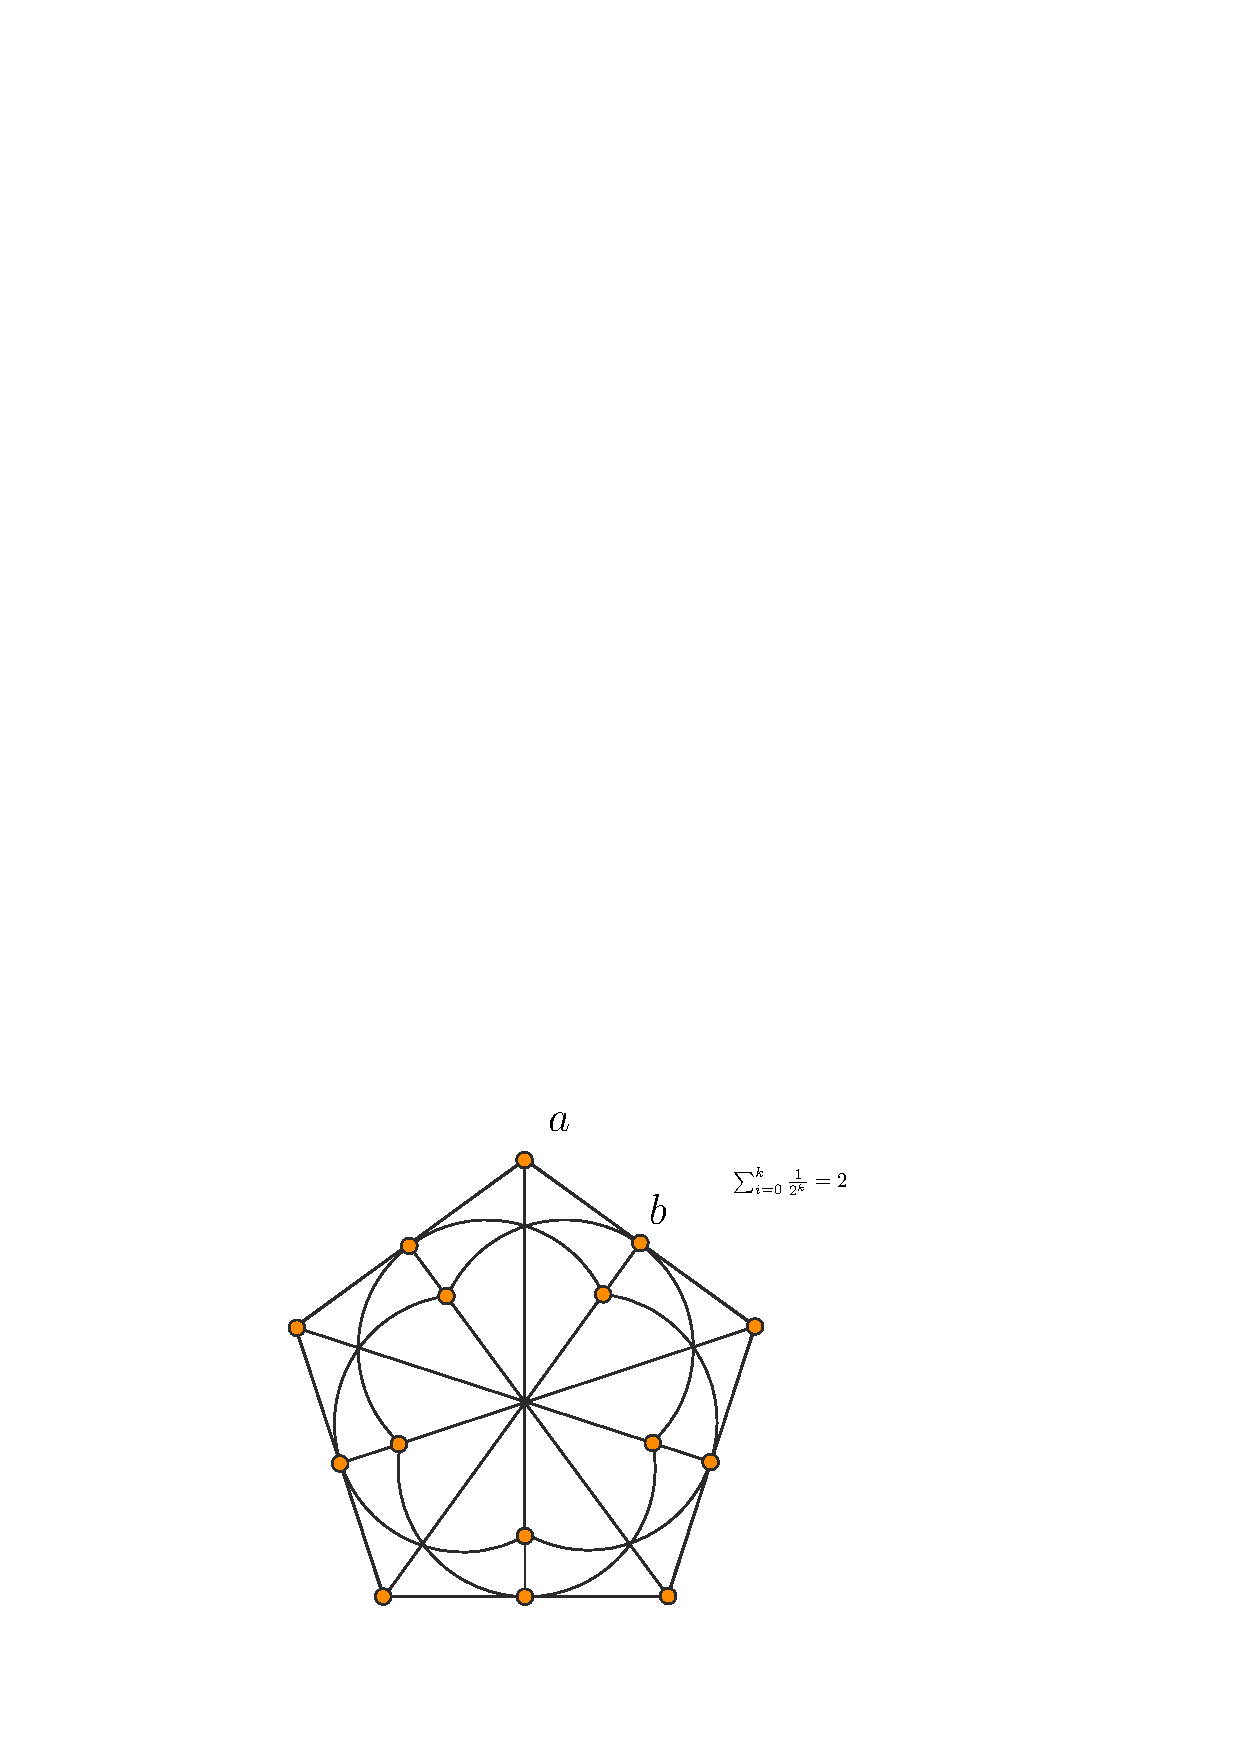
\includegraphics[width=0.5\linewidth]{graf.pdf}
%\end{center}
%\caption{Vhodni podatki.}\label{slika:podatki}
%\end{figure}
%
%\newpage
% Takole se vstavlja tabela.
%
%\begin{table}[h!]
%\caption{Algoritem PLOGBAND}
%\label{tabela:algoritem}
%\fbox{%
%      \parbox{\linewidth}{%
%{\noindent \bf Algoritem PLOGBAND:}
%\vskip 5pt
%\indent Podatka: {\obeylines \indent \indent graf $G = G(V,E)$ na $n$ vozliščih in z $m$ povezavami,
%% \indent \indent nenegativno celo število $L$.}
%\indent \indent $L \in \N$.}
%\begin{enumerate}
%
%\item Za $1 \le j \le L$ naj bodo $p_j$ približno enakomerno
%(geometrijsko) razporejena števila med $1 - 1/\log\log n$ in $1/\log n$.
%Tj., vsa razmerja $p_j/p_{j+1}$ naj bodo približno enaka. (Natančne
%formule so v~razdelku \ref{siroke}, kjer je opisana vložitev naključnih podmnožic.)
%
%\item Uredi vozlišča glede na naraščajoče vrednosti $h(v)$. Vozlišča z enakimi
%vrednostmi $h$ uredi poljubno.
%
%\item Vrni urejeni seznam vozlišč kot linearno ureditev.
%\end{enumerate}
%}}
%\end{table}
%
%\noindent Takole navedemo sliko ali tabelo:
%
%\medskip
%Vse, kar potrebujemo za konec dokaza, je povzeto v Tabeli~\ref{tabela:algoritem}.
%
%\medskip
%Za primer vhodih podatkov glej Sliko~\ref{slika:podatki}.
%
%\medskip
%\noindent Podobno lahko označimo in navajamo razdelke, poglavja, izreke, ipd.
%
%
%\newpage
%Takole lahko zapišemo psevdokodo algoritma:
%\cite{Ukkonen1995}
%\begin{algorithm}[h!]\label{algoritem1}
%\Vhod{Realni matriki $A$ in $B$ velikosti $n\times n$.}
%\Izhod{Matrika $C = A\cdot B$.}
%\caption{Množenje matrik}
%{
%    \Za{$i = 1, \ldots, n$}
%    {
%        \Za{$j = 1, \ldots, n$}
%        {
%            $C[i,j]:= A[i,1]\cdot B[1,j];$
%
%            \Za{$k = 2, \ldots, n$}
%            {
%                $C[i,j]:= C[i,j]+A[i,k]\cdot B[k,j]$;
%            }
%        }
%    }
%    \Ce{$n = 2$}
%    {
%       ne naredi nič
%    }
%    \Repeat{FALSE}{TRUE}
%}
%\Vrni{$C$;}
%\end{algorithm}
%
%
%\chapter{NASLOV POGLAVJA}
%\thispagestyle{fancy}
%
%Takole citiramo spletne vire:~\cite{splet1,splet2,splet3}.\\
%Takole citiramo članke, sprejete v objavo ali v tisku:~\cite{Novak,Novak2,Novak3,Novak4}.\\
%Takole citiramo članke, poslane v objavo:~\cite{Novak5,Novak6}.
%
%%%%%%%%%%%%%%%%%%%%%%%%%%%%%%%%%%% Zaključek %%%%%%%%%%%%%%%%%%%%%%%%%%%%%%%%%%%%%
%\chapter{ZAKLJUČEK}
%\thispagestyle{fancy}
%
%V nekaj stavkih na kratko povzamemo, kaj smo v nalogi obravnavali.
%Po želji lahko navedemo še kakšne dodatne reference za bralca, ki bi ga zanimalo kaj več, ipd.


%%%%%%%%%%%%%%%%%%%%%%%%%%%%%%%% Literatura %%%%%%%%%%%%%%%%%%%%%%%%%%%%%%%%%

 \begin{thebibliography}{99}
\thispagestyle{fancy}
\import{.}{Drugo/Literatura}

% Ena vrstica mora biti tu prazna zaradi pravilnih navedb na strani, kjer so reference citirane.
\end{thebibliography}
\newpage

%%%%%%%%%%%%%%%%%%%%%%%%%%%%%%%%%%%% Priloge %%%%%%%%%%%%%%%%%%%%%%%%%%%%%%%%%%%%%

% Oblikovanje naslovov poglavij (brez Chapter) -> St. poglavja in naslov poglavja
%\makeatletter
%\def\@makechapterhead#1{%
%  \vspace*{30\p@}%
%  { \noindent\LARGE\bf PRILOGA\ \thechapter  \hspace*{0.5cm} \parindent \z@ \raggedright \normalfont
%    \interlinepenalty\@M 
%    \LARGE \bfseries  #1 \par\nobreak
%    \vskip 30\p@
%  }}
%  \makeatother

%\pagestyle{fancyplain}
%\vspace*{\fill}
%     \begin{center}
%          \bf{\Huge{Priloge}}
%     \end{center}
%\vspace*{\fill}
%\thispagestyle{fancy}



  
%\appendix
%\thispagestyle{empty}
%\pagenumbering{gobble}

%\addtocontents{toc}{\setcounter{tocdepth}{-1}}




%\newpage
%\noindent
%\appendices{A Naslov prve priloge}
%\chapter{Naslov prve priloge}
%\textbf{\LARGE{A\hspace{0.8cm}Naslov prve priloge}}\\
%\thispagestyle{empty}
%Tu dodamo prvo prilogo.

% pozor:
% ukaz
% \thispagestyle{empty}
% mora biti prisoten na vsaki strani priloge (da se ne prikaže glava dokumenta)

%\appendices{B Naslov druge priloge}
%\chapter{Naslov druge priloge}
%\thispagestyle{empty}
%Tu dodamo drugo prilogo.

% Pozor:
% ukaz
% \thispagestyle{empty}
% mora biti prisoten na vsaki strani priloge (da se ne prikaže glava dokumenta)

%\addtocontents{toc}{\setcounter{tocdepth}{2}}
\end{document}
